% Sablon pentru realizarea lucrarii de licenta, conform cu recomandarile
% din ghidul de redactare:
% - https://fmi.unibuc.ro/finalizare-studii/
% - https://drive.google.com/file/d/1xj9kZZgTkcKMJkMLRuoYRgLQ1O8CX0mv/view

% Multumiri lui Gabriel Majeri, acest sablon a fost creat pe baza
% codului sursa a lucrarii sale de licenta.
% Codul sursa: https://github.com/GabrielMajeri/bachelors-thesis
% Website: https://www.gabrielmajeri.ro/
%
% Aceast sablon este licentiat sub Creative Commons Attribution 4.0 International License.

\documentclass[12pt, a4paper]{report}

% Suport pentru diacritice și alte simboluri
\usepackage{fontspec}

% Suport pentru mai multe limbi
\usepackage{polyglossia}

% Setează limba textului la română
\setdefaultlanguage{romanian}
% Am nevoie de engleză pentru rezumat
\setotherlanguages{english}

% Indentează și primul paragraf al fiecărei noi secțiuni
\SetLanguageKeys{romanian}{indentfirst=true}

% ====== Despărțirea în silabe la capăt de rând ======
% Documentul nu desparte niciun cuvânt la capăt de rând (fără „admi-nistrator”
% rupt pe două rânduri). Penalizarea maximă pentru cratimă face ca TeX să prefere
% întotdeauna o spațiere ceva mai largă în locul unei despărțiri, iar
% `emergencystretch` îi dă spațiul suplimentar de care are nevoie ca să nu rezulte
% rânduri care depășesc marginea din dreapta.
\hyphenpenalty=10000
\exhyphenpenalty=10000
\tolerance=9999
\emergencystretch=3em

% Suport pentru diferite stiluri de ghilimele
\usepackage{csquotes}

\DeclareQuoteStyle{romanian}
  {\quotedblbase}
  {\textquotedblright}
  {\guillemotleft}
  {\guillemotright}

% Utilizează biblatex pentru referințe bibliografice
% `isbn`/`doi` sunt cerute explicit: elementul de identificare al unei cărți
% (ISBN) și, respectiv, al unui document digital (DOI) trebuie să apară tipărit
% în bibliografie, nu doar să existe în fișierul .bib.
\usepackage[
    maxbibnames=50,
    sorting=nty,
    isbn=true,
    doi=true,
    url=true
]{biblatex}

\addbibresource{bibliography.bib}

% Setează spațiere inter-linie la 1.5
\usepackage{setspace}
\onehalfspacing

% Modificarea geometriei paginii
\usepackage{geometry}

% Include funcțiile de grafică
\usepackage{graphicx}
% Încarcă imaginile din directorul `images`
\graphicspath{{./images/}}

% Permite inserarea unor pagini dintr-un fișier PDF extern (folosit pentru anexă)
\usepackage{pdfpages}

% Diagrame desenate direct în LaTeX (ER, arhitectură)
\usepackage{tikz}
\usetikzlibrary{arrows.meta, positioning, shapes.geometric}

% Listări de cod
\usepackage{listings}
\usepackage{xcolor}

% Stil pentru listările de cod C#
\definecolor{codegray}{rgb}{0.95,0.95,0.95}
\definecolor{codekeyword}{rgb}{0.13,0.29,0.53}
\definecolor{codecomment}{rgb}{0.0,0.5,0.0}
\definecolor{codestring}{rgb}{0.64,0.08,0.08}

\lstdefinestyle{csharpstyle}{
    language=[Sharp]C,
    backgroundcolor=\color{codegray},
    basicstyle=\ttfamily\footnotesize,
    keywordstyle=\color{codekeyword}\bfseries,
    commentstyle=\color{codecomment}\itshape,
    stringstyle=\color{codestring},
    % `columns=fullflexible` + `keepspaces` lasă fiecare caracter la lățimea lui
    % naturală, în loc să-l alinieze pe un caiet de pătrățele: fără această
    % pereche de opțiuni, listările capătă spații parazite în interiorul
    % identificatorilor și al șirurilor de caractere (de exemplu, un URL apare
    % rupt în bucăți: „www . google .com / api”).
    columns=fullflexible,
    keepspaces=true,
    % Liniile din listări sunt deja scrise suficient de scurt cât să încapă în
    % lățimea paginii. Opțiunile de mai jos rămân ca plasă de siguranță: dacă o
    % linie depășește totuși marginea, este ruptă (oriunde, nu doar la spațiu) și
    % continuarea ei este marcată vizibil cu o săgeată.
    breaklines=true,
    breakatwhitespace=false,
    breakindent=2em,
    postbreak=\mbox{\textcolor{gray}{$\hookrightarrow$}\space},
    captionpos=b,
    showstringspaces=false,
    numbers=left,
    numberstyle=\tiny\color{gray},
    numbersep=8pt,
    frame=single,
    framesep=4pt,
    rulecolor=\color{gray!40},
    tabsize=4,
    xleftmargin=12pt
}

\lstset{style=csharpstyle}

% Linkuri interactive în PDF
\usepackage[
    colorlinks,
    linkcolor={black},
    menucolor={black},
    citecolor={black},
    urlcolor={blue}
]{hyperref}

% Comenzi matematice
\usepackage{amsmath}
\usepackage{mathtools}

% Formule matematice
% (definite folosind comenzi standard amsmath/mathtools, nu unicode-math -
% pachetul unicode-math este unul dintre cele mai costisitoare la compilare
% în combinație cu fontspec/polyglossia, iar teza nu conține notație
% matematică ce ar necesita simbolurile Unicode suplimentare oferite de el)
\newcommand{\bigO}[1]{\mathcal{O}\left(#1\right)}
\DeclarePairedDelimiter\abs{\lvert}{\rvert}

% Spațiere mai compactă pentru liste (itemize/enumerate) și pentru titlurile
% de secțiune - reduce numărul de pagini aproape goale rămase la finalul unui
% capitol, fără a modifica vizibil aspectul general al documentului.
\usepackage{enumitem}
\setlist{itemsep=0.15em, parsep=0pt, topsep=0.4em}

\usepackage{titlesec}
\titlespacing*{\section}{0pt}{1.4em plus .2em minus .2em}{0.6em plus .1em}
\titlespacing*{\subsection}{0pt}{1.2em plus .2em minus .2em}{0.5em plus .1em}

% Titlurile de secțiune păstrează formatul implicit al clasei `report`, dar sunt
% aliniate la stânga: un titlu lung se mută integral pe rândul următor, în loc să
% fie despărțit prin cratimă sau întins pe toată lățimea paginii.
\titleformat{\section}{\normalfont\Large\bfseries\raggedright}{\thesection}{1em}{}
\titleformat{\subsection}{\normalfont\large\bfseries\raggedright}{\thesubsection}{1em}{}

% Suport pentru rezumat în două limbi
% Bazat pe https://tex.stackexchange.com/a/70818
\newenvironment{abstractpage}
  {\cleardoublepage\vspace*{\fill}\thispagestyle{empty}}
  {\vfill\cleardoublepage}

\renewenvironment{abstract}[1]
  {\bigskip\selectlanguage{#1}%
   \begin{center}\bfseries\abstractname\end{center}}
  {\par\bigskip}

% Suport pentru anexe
\usepackage{appendix}

% Stiluri diferite de headere și footere
\usepackage{fancyhdr}

% Metadate
\title{CourseHub -- Platformă web pentru conectarea profesorilor cu elevii}
\author{Avramescu Isaac Sebastian}

% Generează variabilele cu @
\makeatletter

\begin{document}

% Front matter
\cleardoublepage
\let\ps@plain

% Pagina de titlu
\begin{titlepage}

% Redu marginile
\newgeometry{left=2cm,right=2cm,bottom=1cm}

\begin{figure}[!htb]
    \centering
    \begin{minipage}{0.2\textwidth}
        
\includegraphics[width=\linewidth]{logo-ub.png}
    \end{minipage}
    \begin{minipage}{0.5\textwidth}
        \large
        \vspace{0.2cm}
        \begin{center}
            \textbf{UNIVERSITATEA DIN BUCUREȘTI}
        \end{center}
        \vspace{0.3cm}
        \begin{center}
            \textbf{
                FACULTATEA DE \\
                MATEMATICĂ ȘI INFORMATICĂ
            }
        \end{center}
    \end{minipage}
    \begin{minipage}{0.2\textwidth}
        
\includegraphics[width=\linewidth]{logo-fmi.png}
    \end{minipage}
\end{figure}

\begin{center}
\textbf{SPECIALIZAREA INFORMATICĂ}
\end{center}

\vspace{1cm}

\begin{center}
\Large \textbf{Lucrare de licență}
\end{center}

\begin{center}
\huge \textbf{\MakeUppercase{\@title}}
\end{center}

\vspace{3cm}

\begin{center}
\large \textbf{Absolvent \\ \@author}
\end{center}

\vspace{0.25cm}

\begin{center}
\large \textbf{Coordonator științific \\ Conf. Univ. Dr. Marius Iulian Mihăilescu}
\end{center}

\vspace{2cm}

\begin{center}
\Large \textbf{București, septembrie 2026}
\end{center}
\end{titlepage}


\restoregeometry

\newgeometry{
    margin=2.5cm
}

\fancypagestyle{main}{
  \fancyhf{}
  \renewcommand\headrulewidth{0pt}
  \fancyhead[C]{}
  \fancyfoot[C]{\thepage}
}

\addtocounter{page}{1}

% Rezumatul
\begin{abstractpage}

\begin{abstract}{romanian}
Lucrarea de față prezintă proiectarea și dezvoltarea aplicației web CourseHub, o
platformă care conectează profesori și elevi într-un spațiu comun de învățare. Obiectivul
principal este construirea unui sistem în care un utilizator își poate crea un profil ca
profesor sau ca elev, poate căuta un partener potrivit după materie, nivel și rol, poate
iniția o colaborare printr-o cerere de colaborare și poate comunica ulterior în timp real,
inclusiv prin partajarea de fișiere și materiale didactice. Platforma a fost dezvoltată
folosind ASP.NET Core 8, Entity Framework Core și SQL Server, cu comunicare
în timp real realizată prin SignalR. Printre funcționalitățile implementate se numără
autentificarea securizată prin cod OTP trimis pe email, un sistem de roluri bazat pe
Identity Roles cu panou de administrare dedicat, protecția formularului de înregistrare
prin reCAPTCHA, încărcarea de avatare și fișiere validate atât din punct de vedere al
tipului, cât și al dimensiunii, precum și o interfață disponibilă integral în limbile română
și engleză. Rezultatele obținute arată o platformă funcțională, cu accent pe securitate,
experiența utilizatorului și posibilitatea de moderare a conținutului, oferind în același
timp un punct de plecare solid pentru extinderi ulterioare.
\end{abstract}

\begin{abstract}{english}
This thesis presents the design and development of the CourseHub web application, a
platform that connects teachers and learners within a shared learning space. The main
objective is to build a system in which a user can create a profile as either a teacher
or a learner, search for a suitable partner by subject, level and role, initiate a collaboration
through a collaboration request, and subsequently communicate in real time, including through
file and teaching material sharing. The platform was developed using ASP.NET Core 8,
Entity Framework Core and SQL Server, with real-time communication implemented
through SignalR. Among the implemented features are secure authentication through
an email OTP code, a role-based system built on Identity Roles with a dedicated admin
panel, registration form protection through reCAPTCHA, avatar and file uploads
validated by both type and size, and a user interface fully available in both Romanian
and English. The results show a functional platform with an emphasis on security,
user experience and content moderation capabilities, while also providing a solid
foundation for future extensions.
\end{abstract}

\end{abstractpage}


\tableofcontents

% Main matter
\cleardoublepage
\pagestyle{main}
\let\ps@plain\ps@main

\chapter{Introducere}

\section{Motivație}

Când un elev lucrează unu la unu cu un profesor potrivit lui, învață mult mai bine
decât la clasă. Problema e cum îl găsește. De obicei totul se rezolvă prin
cunoștințe: întrebi pe cineva, care întreabă pe altcineva, și așa mai departe. Iar
un profesor care vrea să dea meditații n-are unde să își facă un profil, să fie
găsit de elevi și să vorbească apoi cu ei într-un singur loc.

Platformele generaliste de comunicare (rețele sociale, aplicații de mesagerie) nu oferă
structura necesară unei relații profesor-elev: nu există un mod clar de a exprima ce
predai sau ce vrei să înveți, nu există un sistem de conectare bazat pe cerere și acceptare,
iar comunicarea și partajarea materialelor didactice se realizează ad-hoc, fără un istoric
organizat pe fiecare colaborare. Există, așadar, o nevoie clară pentru o platformă dedicată,
care să structureze întregul parcurs: de la crearea unui profil, la găsirea partenerului
potrivit, la comunicarea propriu-zisă.

\section{Context și preliminarii}

Platformele educaționale existente se împart, în linii mari, în două categorii:
platforme de cursuri înregistrate, fără interacțiune personalizată, și platforme de
mediere între tutori și elevi, orientate comercial. Foarte puține pun accentul pe
comunicarea directă, în timp real, odată ce colaborarea a fost stabilită, sau pe
posibilitatea profesorului de a trimite un material de lucru chiar în conversația
în care discută cu elevul.

CourseHub este gândit ca o soluție dedicată acestei nevoi: nu un magazin de cursuri,
ci un spațiu în care oricine se poate înregistra ca persoană care vrea să predea sau
să învețe, poate căuta un partener după criterii clare (rol, nivel, materie), poate
iniția o colaborare printr-un mecanism explicit de cerere și acceptare, iar apoi poate
comunica prin chat în timp real, inclusiv prin partajarea de fișiere.

\section{Obiectivele lucrării}

Obiectivul principal al acestei lucrări este proiectarea și implementarea platformei
CourseHub, folosind ASP.NET Core 8 și tehnologii moderne asociate ecosistemului
.NET. Obiectivele specifice sunt:

\begin{itemize}
    \item construirea unui sistem de înregistrare securizat, cu verificare a adresei de
    email printr-un cod de unică folosință (OTP) și protecție a formularului de
    înregistrare printr-un mecanism de tip \emph{CAPTCHA};
    \item implementarea unui flux de completare a profilului (\emph{wizard}) prin care
    utilizatorul își alege rolul (profesor sau elev), detaliile relevante rolului ales
    (nivel de experiență, respectiv nivel de studii) și materiile de interes;
    \item dezvoltarea unui sistem de căutare și filtrare a utilizatorilor după rol, nivel
    și materie;
    \item construirea unui mecanism explicit de conectare, bazat pe cereri de colaborare
    trimise de un elev unui profesor și acceptate sau respinse de acesta;
    \item implementarea unui sistem de mesagerie în timp real, folosind SignalR,
    cu suport pentru partajarea de fișiere de către profesori către elevii cu care
    colaborează;
    \item construirea unui sistem de roluri real, bazat pe \emph{ASP.NET Identity Roles},
    și a unui panou de administrare care permite gestionarea utilizatorilor, a materiilor
    disponibile pe platformă, precum și moderarea conținutului trimis prin chat;
    \item realizarea unei interfețe complet localizate, disponibilă atât în limba română,
    cât și în limba engleză.
\end{itemize}

\section{Contribuția personală}

Toate componentele platformei CourseHub -- modelul de date, logica din controllere,
interfața, autentificarea și verificarea prin OTP, sistemul de roluri, panoul de
administrare, mesageria în timp real și localizarea -- au fost proiectate și
implementate integral ca parte a acestei lucrări, cu accent pe corectitudinea
fluxurilor de autorizare, pe validarea riguroasă a datelor introduse de utilizator
și pe o experiență de utilizare coerentă în ambele limbi.

\section{Structura lucrării}

Capitolul 2 analizează cerințele funcționale și nefuncționale, împreună cu actorii
implicați, iar capitolul 3 prezintă tehnologiile folosite. Capitolul 4 descrie
modelarea bazei de date și arhitectura sistemului, capitolul 5 detaliază
implementarea, capitolul 6 aspectele de securitate, iar capitolul 7 metodologia de
testare. Capitolul 8 conține concluziile, limitările și direcțiile de dezvoltare
ulterioară.

\chapter{Analiza cerințelor}

\section{Introducere}

Înainte să încep să scriu cod, a trebuit să stabilesc cine folosește platforma și
ce trebuie să poată face fiecare. În capitolul ăsta trec prin tipurile de
utilizatori și prin cerințele care au ieșit din problema descrisă mai devreme.

\section{Actorii sistemului}

Platforma distinge patru tipuri de actori, ultimele trei reprezentate tehnic prin
roluri reale din \emph{ASP.NET Identity}: \textbf{Vizitator} (persoană
neautentificată, poate accesa pagina principală, se poate înregistra sau
autentifica), \textbf{Elev} (rol \texttt{Learn}, caută un profesor, trimite cereri
de colaborare, comunică prin chat cu profesorii cu care colaborează),
\textbf{Profesor} (rol \texttt{Teach}, poate fi găsit de elevi, acceptă sau
respinge cereri de colaborare, poate trimite fișiere elevilor cu care
colaborează) și \textbf{Administrator} (rol \texttt{Admin}, gestionează conturile,
blocările și materiile disponibile, moderează mesajele).

Fiecare cont primește, în plus, rolul implicit \texttt{User} la înregistrare.
Acesta nu influențează nicio funcționalitate vizibilă -- există exclusiv pentru
vizibilitate administrativă, ca un administrator să poată confirma din tabela de
roluri că un cont este un membru înregistrat obișnuit.

\section{Cerințe funcționale}

\begin{itemize}
    \item Înregistrare cu nume de utilizator, email și parolă; contul rămâne
    neconfirmat până la introducerea corectă a unui cod OTP trimis pe email.
    \item După confirmare, utilizatorul parcurge un flux de completare a profilului
    în trei pași: alegerea rolului, detaliile specifice rolului (vârstă, gen, nivel
    de studii/experiență) și selectarea a până la trei materii de interes.
    \item Căutarea altor utilizatori după nume, rol, nivel și materie.
    \item Trimiterea unei cereri de colaborare de la elev către profesor; acceptare,
    respingere sau anulare (cât timp e în așteptare) a cererii.
    \item Comunicare prin chat în timp real între utilizatorii care colaborează, cu
    posibilitatea profesorului de a atașa fișiere (documente, imagini, prezentări)
    conversației, și un indicator de mesaje necitite în bara de navigare.
    \item Editarea profilului propriu (biografie, avatar, materii, nivel); modificările
    sensibile (nume de utilizator, email) necesită reconfirmare prin cod OTP.
    \item Administrare: promovare/retrogradare a rolului de administrator, blocare
    temporară (1 zi, 7 zile, 1 lună) sau permanentă, ștergere de cont, gestionarea
    materiilor disponibile.
\end{itemize}

\section{Cerințe nefuncționale}

\begin{itemize}
    \item \textbf{Securitate}: parolele nu sunt stocate în clar (gestionate de
    ASP.NET Identity ca \emph{hash}); fișierele încărcate sunt validate după
    extensie și dimensiune; acțiunile administrative sunt restricționate exclusiv
    rolului \texttt{Admin}, verificat de framework, nu doar ascuns din interfață;
    toate cererile care modifică starea aplicației sunt însoțite de un token
    antiforgery validat pe server.
    \item \textbf{Localizare}: interfața este disponibilă integral în română și
    engleză, comutabilă fără reîncărcare manuală și fără autentificare.
    \item \textbf{Utilizabilitate}: interfața este responsivă și accesibilă atât
    pe desktop, cât și pe dispozitive mobile.
    \item \textbf{Extensibilitate}: arhitectura modulară (controllere separate
    pentru căutare, colaborări, cereri, chat, administrare) permite adăugarea de
    noi funcționalități fără a afecta modulele existente.
    \item \textbf{Fiabilitate}: acțiunile ireversibile (ștergere, blocare
    permanentă) sunt limitate prin verificări explicite -- un administrator nu
    își poate șterge sau bloca propriul cont, iar niciun administrator nu poate
    fi blocat sau șters de altul.
    \item \textbf{Mentenabilitate}: evoluția schemei bazei de date este gestionată
    exclusiv prin migrații Entity Framework Core, trasabile și reproductibile pe
    orice mediu nou.
\end{itemize}

\chapter{Tehnologii și instrumente utilizate}

\section{Introducere}

Platforma CourseHub a fost construită folosind ecosistemul .NET, în jurul
framework-ului \emph{ASP.NET Core 8}. Această secțiune prezintă principalele
tehnologii folosite și motivele pentru care au fost alese.

\section{ASP.NET Core 8 și Entity Framework Core}

ASP.NET Core este un framework \emph{cross-platform} și \emph{open-source},
dezvoltat de Microsoft, dedicat construirii de aplicații web și servicii
API~\cite{aspnetcore-docs}. Aplicația CourseHub folosește
modelul \emph{MVC} (\emph{Model-View-Controller}), un tipar arhitectural propus
inițial pentru interfețe grafice și adaptat ulterior aplicațiilor
web, pentru partea principală a aplicației și \emph{Razor Pages} pentru fluxurile
legate de autentificare (\texttt{Areas/Identity}), respectând convenția folosită
de șabloanele oficiale ale platformei Identity. Structura proiectului urmează
organizarea standard \texttt{Models}/\texttt{Controllers}/\texttt{Views},
completată de un director \texttt{Services} pentru componente reutilizabile
(email, verificarea reCAPTCHA, curățarea codurilor OTP expirate). Limbajul
folosit este C\#~\cite{csharp-docs}.

Persistența datelor este realizată prin \emph{Entity Framework Core}, ORM-ul
oficial pentru .NET~\cite{efcore-docs}. Toate entitățile platformei
(\texttt{ApplicationUser}, \texttt{Message}, \texttt{HireRequest}, \texttt{Topic},
\texttt{OtpCode}) sunt mapate pe o bază de date \emph{SQL Server}~\cite{sqlserver-docs},
iar evoluția schemei este gestionată exclusiv prin \emph{migrații}: fiecare
modificare a modelului de date este însoțită de o migrație dedicată, aplicată
prin comanda \texttt{Update-Database}.

\section{ASP.NET Identity și sistemul de roluri}

Autentificarea și gestionarea utilizatorilor sunt realizate prin \emph{ASP.NET
Identity}~\cite{identity-docs}, extins cu suport pentru roluri reale
(\texttt{RoleManager<IdentityRole>})~\cite{identity-roles-docs}: \texttt{User}
(atribuit automat oricărui cont), \texttt{Teach}, \texttt{Learn} și \texttt{Admin}.
Rolurile \texttt{Teach}/\texttt{Learn} sunt menținute sincronizat atât în câmpul
\texttt{Role} al entității \texttt{ApplicationUser} (folosit de restul aplicației
pentru afișare și filtrare), cât și în tabela reală \texttt{AspNetRoles}, ceea ce
permite verificări stricte de tipul \texttt{[Authorize(Roles = "Admin")]} pentru
panoul de administrare.

\section{SignalR -- comunicare în timp real}

Chat-ul dintre profesor și elev este implementat cu \emph{SignalR}, biblioteca
oficială pentru comunicare bidirecțională în timp real peste
\emph{WebSockets}~\cite{signalr-docs, websocket-rfc}, cu \emph{fallback} automat
la alte transporturi când este necesar. \texttt{ChatHub} expune metoda
\texttt{SendMessage}, apelată de client prin conexiunea SignalR, care
redirecționează mesajul instantaneu către destinatar, în paralel cu persistarea
acestuia printr-un apel API separat, ale cărui endpoint-uri urmează principiile
arhitecturale REST~\cite{fielding-rest}.

\section{reCAPTCHA}

Formularul de înregistrare este protejat împotriva înregistrărilor automate
(\emph{bot}) prin \emph{Google reCAPTCHA v2}~\cite{recaptcha-docs}. Verificarea
token-ului trimis de client este realizată exclusiv pe server, printr-un apel
către serviciul \texttt{siteverify} al Google, înainte ca un cont nou să fie
creat efectiv.

\section{Localizare}

Interfața este disponibilă integral în română și engleză, folosind sistemul
nativ de localizare din ASP.NET Core (\texttt{IStringLocalizer},
\texttt{IViewLocalizer} și fișiere de resurse \texttt{.resx})~\cite{localization-docs}.
Limba română este cea implicită; comutarea se face printr-un \emph{cookie}
setat de un controller dedicat, fără reîncărcare manuală și fără autentificare.

\section{Alte tehnologii și instrumente}

\begin{itemize}
    \item \textbf{SMTP} pentru codurile OTP și notificările prin email;
    \item \textbf{Bootstrap 5}~\cite{bootstrap-docs}, peste care a fost construit
    un sistem propriu de stiluri (culori, carduri, animații);
    \item \textbf{Git}~\cite{git-docs} și \textbf{Visual Studio} pentru controlul
    versiunilor, dezvoltare și depanare;
    \item \textbf{SQL Server LocalDB} ca sistem de gestiune a bazei de date în
    mediul de dezvoltare;
    \item \textbf{Postman}, pentru testarea manuală a endpoint-urilor API (de
    exemplu \texttt{/api/messages/upload-file}), independent de formular;
    \item \textbf{LaTeX} (XeLaTeX), pentru redactarea prezentei lucrări, necesar
    pentru suportul diacriticelor prin \texttt{fontspec} și \texttt{polyglossia}.
\end{itemize}

\chapter{Modelarea bazei de date și arhitectura sistemului}

\section{Introducere}

Aici arăt cum arată baza de date din spatele aplicației: ce entități am definit,
cum se leagă între ele și cum am împărțit codul pe module.

\section{Modelarea bazei de date}

Baza de date este construită pe un model relațional~\cite{elmasri-navathe},
gestionat prin Entity Framework Core. Pe lângă entitățile proprii aplicației, schema
include și tabelele standard generate de \emph{ASP.NET Identity}
(\texttt{AspNetUsers}, \texttt{AspNetRoles} etc.), entitatea \texttt{ApplicationUser}
extinzând clasa \texttt{IdentityUser}.

\subsection{Entități principale}

Denumirile claselor păstrează terminologia engleză folosită la implementare
(\texttt{Topic} pentru materie, \texttt{HireRequest} pentru cererea de colaborare),
în timp ce textul lucrării și interfața folosesc termenii românești.

\begin{description}
    \item[ApplicationUser] reprezintă un cont de utilizator; extinde \texttt{IdentityUser}
    cu câmpurile \texttt{Bio}, \texttt{Role} (\texttt{"Teach"} sau \texttt{"Learn"}),
    \texttt{EducationLevel}, \texttt{TeachingLevel}, \texttt{Age}, \texttt{Gender},
    \texttt{SelectedTopics} (identificatorii materiilor alese, separați prin virgulă),
    \texttt{AvatarPath} și \texttt{BannedUntil} (data până la care contul e blocat).
    \item[Message] reprezintă un mesaj din conversația dintre doi utilizatori: conține
    \texttt{SenderId}, \texttt{ReceiverId}, \texttt{Content}, \texttt{Timestamp},
    \texttt{IsRead}, precum și câmpurile opționale \texttt{FilePath}, \texttt{FileName}
    și \texttt{FileSize}, populate atunci când mesajul conține un fișier atașat.
    \item[HireRequest] reprezintă o cerere de colaborare trimisă de un elev unui profesor:
    conține \texttt{RequesterId}, \texttt{TargetId}, \texttt{IsAccepted} și
    \texttt{RequestedAt}.
    \item[Topic] reprezintă o materie (de exemplu, Matematică, Programare);
    conține \texttt{Name} și \texttt{Description}.
    \item[OtpCode] reprezintă un cod de unică folosință generat pentru verificarea
    email-ului sau confirmarea unei modificări sensibile a profilului; conține
    \texttt{UserId}, \texttt{Code} și \texttt{ExpirationTime}.
\end{description}

\subsection{Relații importante}

Figura~\ref{fig:er-diagram} prezintă relațiile principale dintre entități.

\begin{figure}[h]
\centering
\begin{tikzpicture}[
    box/.style={draw, rectangle, rounded corners=2pt, minimum width=2.6cm, minimum height=0.8cm, align=center, font=\small},
    >=Stealth
]
\node[box] (user) {ApplicationUser};
\node[box, right=3.6cm of user, yshift=2.4cm] (message) {Message};
\node[box, right=3.6cm of user, yshift=0.8cm] (hire) {HireRequest};
\node[box, right=3.6cm of user, yshift=-0.8cm] (otp) {OtpCode};
\node[box, right=3.6cm of user, yshift=-2.4cm] (topic) {Topic};
\node[box, above=1.8cm of user] (role) {AspNetRoles};

\draw[->] (user) -- (message) node[midway, above, sloped, font=\tiny] {1..n (Sender / Receiver)};
\draw[->] (user) -- (hire) node[midway, above, sloped, font=\tiny] {1..n (Requester / Target)};
\draw[->] (user) -- (otp) node[midway, above, sloped, font=\tiny] {1..n};
\draw[->] (user) -- (topic) node[midway, above, sloped, font=\tiny] {n..n (la nivel de aplicație)};
\draw[->] (user) -- (role) node[midway, right, font=\tiny] {n..n};
\end{tikzpicture}
\caption{Diagrama entitate-relație simplificată a bazei de date CourseHub}
\label{fig:er-diagram}
\end{figure}

Un utilizator (\texttt{ApplicationUser}) poate fi atât expeditor, cât și destinatar al
mai multor mesaje, atât solicitant (elev), cât și țintă (profesor) a mai multor cereri
de colaborare, și poate avea mai multe coduri OTP și roluri asociate. Dintre acestea,
doar legătura cu \texttt{HireRequest} este materializată printr-o cheie externă
propriu-zisă; relația cu \texttt{OtpCode} este menținută la nivel de aplicație, prin
câmpul \texttt{UserId}.

Relația dintre \texttt{ApplicationUser} și \texttt{Topic} este, de asemenea, implementată
intenționat la nivel de aplicație, prin lista de identificatori din \texttt{SelectedTopics},
și nu printr-o tabelă de legătură: un utilizator poate selecta cel mult trei materii, iar
operațiile necesare sunt suficient de simple pentru a nu justifica o entitate suplimentară.

\section{Arhitectura logică a sistemului}

CourseHub este structurată modular, fiecare controller acoperind o arie de
responsabilitate clară:

\begin{itemize}
    \item \textbf{Identity (Areas/Identity)}: înregistrare, autentificare, verificare OTP,
    resetarea parolei, gestionarea profilului propriu (\texttt{Manage});
    \item \textbf{SearchController}: căutarea și filtrarea utilizatorilor;
    \item \textbf{HireController}: trimiterea, acceptarea, anularea cererilor de colaborare;
    \item \textbf{ConnectionsController}: afișarea listei de colaborări active (elevi, respectiv
    profesori, în funcție de rol);
    \item \textbf{ChatController} și \textbf{ChatHub}: afișarea istoricului unei conversații
    și, respectiv, livrarea mesajelor în timp real prin SignalR;
    \item \textbf{MessagesController}: lista mesajelor primite, cu conversațiile recente ale utilizatorului;
    \item \textbf{AdminController}: panoul de administrare (utilizatori, roluri, blocări,
    materii, moderarea mesajelor).
\end{itemize}

Figura~\ref{fig:arhitectura} ilustrează fluxul general al unei cereri prin sistem.

\begin{figure}[h]
\centering
\begin{tikzpicture}[
    box/.style={draw, rectangle, minimum width=3.4cm, minimum height=0.9cm, align=center, font=\small},
    >=Stealth
]
\node[box] (browser) {Interfață web\\(Razor Views, JS)};
\node[box, below=1.2cm of browser] (mvc) {ASP.NET Core\\(Controllere, Servicii)};
\node[box, below left=1.2cm and 2.2cm of mvc] (db) {SQL Server\\(Entity Framework Core)};
\node[box, below right=1.2cm and 2.2cm of mvc] (hub) {SignalR Hub\\(ChatHub)};

\draw[->] (browser) -- (mvc) node[midway, right, font=\tiny] {HTTP(S)};
\draw[->] (mvc) -- (db) node[midway, left, font=\tiny] {EF Core};
\draw[<->] (browser) -- (hub) node[midway, right, font=\tiny] {WebSocket};
\draw[->] (hub) -- (mvc) node[midway, below, font=\tiny] {};
\end{tikzpicture}
\caption{Arhitectura logică a platformei CourseHub}
\label{fig:arhitectura}
\end{figure}

\subsection{Fluxuri funcționale principale}

Parcursul unui utilizator leagă modulele de mai sus într-un singur lanț: se
înregistrează printr-un formular protejat de reCAPTCHA și își confirmă contul cu
un cod OTP, parcurge apoi fluxul de trei pași prin care își definește rolul,
detaliile și materiile de interes, caută un partener potrivit și îi trimite o
cerere de colaborare, iar din momentul acceptării cei doi comunică prin chat în
timp real, profesorul putând atașa suplimentar fișiere. În paralel,
administratorul gestionează conturile, rolurile, blocările și materiile
disponibile pe platformă.

\chapter{Implementarea funcționalităților majore}

\section{Introducere}

Acest capitol detaliază implementarea principalelor funcționalități ale platformei
CourseHub: gestionarea conturilor și autentificarea, fluxul de completare a
profilului, căutarea și sistemul de cereri de colaborare, mesageria în timp real cu
partajare de fișiere, panoul de administrare și sistemul de localizare.

\section{Gestionarea utilizatorilor}

Entitatea \texttt{ApplicationUser} extinde clasa \texttt{IdentityUser} din
ASP.NET Identity cu proprietăți specifice domeniului:

\begin{lstlisting}[caption={Extinderea entității de utilizator (fragment)}]
public class ApplicationUser : IdentityUser
{
    public string? Bio { get; set; }
    public string? Role { get; set; }
    public string? EducationLevel { get; set; }
    public string? TeachingLevel { get; set; }
    public int? Age { get; set; }
    public string? Gender { get; set; }
    public string? SelectedTopics { get; set; }
    public string? AvatarPath { get; set; }
    public DateTime? BannedUntil { get; set; }
}
\end{lstlisting}

Câmpul \texttt{BannedUntil} ilustrează o decizie de proiectare deliberată: în loc
de un câmp boolean separat (\texttt{IsBanned}), o singură dată nullable acoperă
toate cazurile -- \texttt{null} înseamnă cont neblocat, o dată din viitor înseamnă
blocare temporară, iar \texttt{DateTime.MaxValue} este folosit convențional pentru
blocare permanentă. Verificarea „este blocat” se reduce, în orice context, la o
singură comparație: \texttt{BannedUntil > DateTime.UtcNow}.

\section{Autentificarea și verificarea prin OTP}

Înregistrarea unui cont nou nu autentifică imediat utilizatorul. După crearea
contului, se generează un cod numeric de 6 cifre, stocat împreună cu un termen de
expirare în tabela \texttt{OtpCode}, iar codul este trimis pe adresa de email
indicată. Contul rămâne neconfirmat (\texttt{EmailConfirmed = false}) până la
introducerea corectă a codului pe pagina dedicată de verificare. Același mecanism
este reutilizat pentru confirmarea modificărilor sensibile ale profilului
(schimbarea numelui de utilizator sau a adresei de email).

\section{Fluxul de completare a profilului}

Imediat după confirmarea contului, utilizatorul este direcționat către un flux de
completare a profilului, organizat în trei pași: alegerea rolului, completarea
detaliilor specifice rolului ales și selectarea materiilor de interes. O atenție
particulară a fost acordată transmiterii corecte a rolului între pași -- valoarea
aleasă la primul pas trebuie păstrată într-un câmp ascuns al formularului, altfel
serverul nu ar putea decide dacă trebuie salvat nivelul de educație sau nivelul de
predare. La finalul primului pas, rolul ales este scris atât în câmpul
\texttt{Role} al utilizatorului, cât și în tabela reală de roluri Identity:

\begin{lstlisting}[caption={Sincronizarea rolului domeniu cu rolul Identity}]
user.Role = Wizard.Role;
await _userManager.UpdateAsync(user);

var otherRole = Wizard.Role == "Teach" ? "Learn" : "Teach";
if (await _userManager.IsInRoleAsync(user, otherRole))
    await _userManager.RemoveFromRoleAsync(user, otherRole);
if (!await _userManager.IsInRoleAsync(user, Wizard.Role))
    await _userManager.AddToRoleAsync(user, Wizard.Role);
\end{lstlisting}

\section{Căutarea și sistemul de cereri de colaborare}

Căutarea permite filtrarea utilizatorilor după nume, rol, nivel de experiență
și materie, excluzând întotdeauna conturile cu rol de administrator din rezultate,
indiferent de valoarea câmpului \texttt{Role} pe care acestea o au. Un elev poate
trimite unei persoane cu rol de profesor o cerere de colaborare
(\texttt{HireRequest}); profesorul o poate accepta sau respinge din pagina
proprie de cereri, iar elevul poate vizualiza starea propriilor cereri trimise și
le poate anula cât timp sunt în așteptare. Odată o cerere acceptată, cei doi
utilizatori devin parteneri și pot iniția o conversație.

\section{Mesageria în timp real și partajarea fișierelor}

Comunicarea dintre utilizatori se realizează printr-un chat cu livrare
instantanee, implementat cu SignalR. Hub-ul expune o singură metodă, apelată de
client pentru a trimite un mesaj text:

\begin{lstlisting}[caption={ChatHub -- livrarea mesajelor în timp real}]
public class ChatHub : Hub
{
    public async Task SendMessage(
        string senderId, string receiverId, string message)
    {
        await Clients.User(receiverId)
            .SendAsync("ReceiveMessage", senderId, message);
    }
}
\end{lstlisting}

În paralel cu livrarea prin SignalR, clientul trimite mesajul și către un
endpoint API dedicat, responsabil de persistarea acestuia în baza de date --
separarea celor două căi permite ca istoricul conversației să rămână disponibil
chiar dacă unul dintre utilizatori nu este conectat în momentul trimiterii.

Profesorii pot, suplimentar, atașa fișiere conversației. Restricția este aplicată
exclusiv pe server, nu doar prin ascunderea butonului de atașare din interfață
pentru elevi: tipul fișierului este verificat printr-o listă albă de extensii,
dimensiunea este limitată, iar numele fișierului salvat pe disc este generat
aleator (\texttt{Guid.NewGuid}), pentru a preveni suprascrierea accidentală a
unui fișier existent cu același nume.

\section{Panoul de administrare}

Panoul de administrare este restricționat prin atributul
\texttt{[Authorize(Roles = "Admin")]}, aplicat la nivel de controller -- framework-ul
respinge orice cerere provenită de la un utilizator neautorizat, înainte ca vreo
linie de cod din interior să se execute.

Administratorul poate promova sau retrograda alți utilizatori, poate șterge un
cont (împreună cu toate mesajele, cererile de colaborare, codurile OTP și avatarul
asociate) și poate bloca temporar sau permanent un cont:

\begin{lstlisting}[caption={Aplicarea unei blocări (fragment din AdminController)}]
switch (duration)
{
    case "1d": user.BannedUntil = DateTime.UtcNow.AddDays(1); break;
    case "7d": user.BannedUntil = DateTime.UtcNow.AddDays(7); break;
    case "1m": user.BannedUntil = DateTime.UtcNow.AddMonths(1); break;
    case "permanent": user.BannedUntil = DateTime.MaxValue; break;
    case "unban": user.BannedUntil = null; break;
}
\end{lstlisting}

Un administrator nu se poate bloca sau șterge pe sine, iar niciun administrator
nu poate fi blocat sau șters de un alt administrator, pentru a preveni pierderea
accidentală a accesului la panoul de administrare. Pentru moderare, administratorul poate
vizualiza, pentru orice utilizator, lista completă a mesajelor trimise de acesta.

\section{Sistemul de localizare}

Textele din interfață sunt extrase în fișiere de resurse (\texttt{.resx}),
organizate în oglindă cu structura de directoare a vizualizărilor, iar textul
românesc este folosit direct drept cheie de resursă:

\begin{lstlisting}[caption={Exemplu de utilizare a localizării într-o vizualizare}]
<h1>@Localizer["Panou de administrare"]</h1>
\end{lstlisting}

Limba activă este determinată printr-un \emph{cookie} setat de un controller
dedicat, apelat la comutarea de limbă din bara de navigare; schimbarea limbii nu
necesită autentificare și este păstrată între sesiuni.

\chapter{Securitate}

\section{Introducere}

Securitatea nu e o funcționalitate pe care o adaugi la final, ci ceva ce trebuie
avut în minte peste tot. De aceea, pentru fiecare formular, încărcare de fișier
și acțiune de administrare m-am întrebat același lucru: ce s-ar întâmpla dacă
cineva ar apela-o direct, fără să treacă prin interfață~\cite{owasp-top10}?

\section{Autentificare și parole}

Parolele nu sunt niciodată stocate în clar; gestionarea lor este delegată
componentei \texttt{PasswordHasher} din ASP.NET Identity~\cite{identity-docs},
care aplică \emph{hashing} cu \emph{salt} unic per utilizator, în linie cu
recomandările privind gestionarea autentificatorilor de tip memorat-secret
publicate de NIST~\cite{nist-800-63b}.

Autentificarea unui cont blocat este respinsă înainte ca sesiunea să fie creată.
Pentru a evita confirmarea existenței unui cont blocat unui atacator care nu
cunoaște parola corectă, verificarea parolei se face separat de autentificarea
efectivă -- mesajul de blocare apare exclusiv când parola introdusă este corectă:

\begin{lstlisting}[caption={Verificarea blocării unui cont, ulterior validării parolei}]
var passwordCheck = await _signInManager.CheckPasswordSignInAsync(
    user, Input.Password, lockoutOnFailure: false);

if (passwordCheck.Succeeded)
{
    if (user.BannedUntil.HasValue &&
        user.BannedUntil.Value > DateTime.UtcNow)
    {
        ModelState.AddModelError(string.Empty, banMessage);
        return Page();
    }
    await _signInManager.SignInAsync(user, isPersistent: false);
    return LocalRedirect(returnUrl);
}
\end{lstlisting}

\section{Autorizare bazată pe roluri}

Panoul de administrare, precum și fiecare acțiune sensibilă din
\texttt{AdminController} (blocare, ștergere, promovare la rolul de administrator,
gestionarea materiilor) sunt protejate prin \texttt{[Authorize(Roles = "Admin")]}
~\cite{identity-roles-docs}, verificat de \emph{middleware}-ul de autorizare al
ASP.NET Core, înaintea execuției oricărui cod din controller. Aceeași filosofie
a fost aplicată restricțiilor de domeniu care nu se mapează pe un rol Identity:
doar un utilizator cu \texttt{Role = "Teach"} poate atașa fișiere unei
conversații, verificare realizată în endpoint-ul de încărcare.

\section{Protecția formularului de înregistrare}

Formularul de înregistrare este protejat prin \emph{Google reCAPTCHA
v2}~\cite{recaptcha-docs}. Token-ul generat de widget-ul din pagină este trimis
către server și verificat printr-un apel către serviciul oficial de validare al
Google, înainte ca vreun cont să fie creat:

\begin{lstlisting}[caption={Verificarea token-ului reCAPTCHA (fragment)}]
public async Task<bool> VerifyAsync(
    string? recaptchaResponse, string? remoteIp)
{
    if (string.IsNullOrWhiteSpace(recaptchaResponse))
        return false;

    var response = await client.PostAsync(
        "https://www.google.com/recaptcha/api/siteverify",
        new FormUrlEncodedContent(parameters));

    var json = await response.Content.ReadAsStringAsync();
    using var doc = JsonDocument.Parse(json);
    return doc.RootElement.TryGetProperty("success", out var s)
           && s.GetBoolean();
}
\end{lstlisting}

Dacă cheia secretă nu este configurată, verificarea eșuează implicit (\emph{fail
closed}) -- înregistrarea rămâne blocată până la configurarea corectă, în loc să
permită tuturor înregistrărilor să treacă nevalidate.

\section{Validarea fișierelor încărcate}

Atât avatarele de profil, cât și fișierele atașate conversațiilor sunt validate
pe server, nu doar prin atributul \texttt{accept} al elementului HTML de tip
fișier (ușor de ocolit): tipul este verificat printr-o listă albă de extensii,
dimensiunea este limitată explicit, iar numele fișierului salvat pe disc este
generat aleator, pentru a preveni atât suprascrierea accidentală a unui fișier
existent, cât și deducerea, din nume, a provenienței acestuia.

\section{Restricționarea accesului la conversații}

O conversație există numai între doi utilizatori legați printr-o cerere de
colaborare acceptată. Interfața respectă regula în mod natural -- butonul de chat
apare exclusiv în lista de colaborări --, dar ea nu poate rămâne doar acolo: un
utilizator autentificat ar putea deschide manual adresa unei conversații cu orice
cont, indicând identificatorul acestuia în URL. Verificarea este, prin urmare,
repetată pe server:

\begin{lstlisting}[caption={Verificarea existenței unei colaborări acceptate}]
var areConnected = await _context.HireRequests.AnyAsync(h =>
    h.IsAccepted &&
    ((h.RequesterId == currentUserId && h.TargetId == userId) ||
     (h.RequesterId == userId && h.TargetId == currentUserId)));

if (!areConnected) return Forbid();
\end{lstlisting}

Aceeași condiție este aplicată atât în endpoint-ul care persistă un mesaj text,
cât și în cel de încărcare a fișierelor.

\section{Protecția împotriva atacurilor CSRF}

Un atac de tip \emph{Cross-Site Request Forgery} exploatează faptul că browser-ul
atașează automat \emph{cookie}-ul de sesiune oricărei cereri către aplicație,
inclusiv uneia inițiate de pe un site străin: o pagină ostilă poate trimite, în
numele unui administrator autentificat, o cerere de ștergere a unui
cont~\cite{owasp-top10}.

Contramăsura standard este un \emph{token} unic per sesiune, inclus în fiecare
formular și validat la primirea cererii. În ASP.NET Core, paginile Razor îl
validează automat, în timp ce controllerele MVC nu o fac decât dacă li se cere
explicit -- exact categoria de acțiuni sensibile din \texttt{AdminController} și
\texttt{HireController}. Validarea a fost, de aceea, activată global:

\begin{lstlisting}[caption={Activarea globală a validării token-ului antiforgery}]
builder.Services.AddAntiforgery(options =>
    options.HeaderName = "RequestVerificationToken");

builder.Services.AddControllersWithViews(options =>
{
    options.Filters.Add(new AutoValidateAntiforgeryTokenAttribute());
});
\end{lstlisting}

Formularele aplicației sunt generate prin \emph{tag helper}-ul de formular, care
include deja token-ul ca un câmp ascuns, deci nicio vizualizare nu a trebuit
modificată. Singurele două cereri care nu provin dintr-un formular -- trimiterea
unui mesaj și încărcarea unui fișier -- transmit token-ul printr-un antet HTTP.

\section{Prevenirea falsificării expeditorului unui mesaj}

Endpoint-ul API prin care se persistă un mesaj nu are voie să aibă încredere în
identificatorul de expeditor trimis de client; acesta este întotdeauna suprascris
cu identitatea utilizatorului autentificat:

\begin{lstlisting}[caption={Suprascrierea expeditorului cu identitatea autentificată}]
var senderId = _userManager.GetUserId(User);
if (senderId == null) return Unauthorized();

message.SenderId = senderId;
\end{lstlisting}

Fără această verificare, un utilizator autentificat ar fi putut construi manual
o cerere HTTP care să pară provenită de la un alt cont.

\section{Protecția integrității datelor și a rolului de administrator}

Ștergerea unui cont elimină explicit toate înregistrările care fac referire la
acel utilizator -- mesajele trimise și primite, cererile de colaborare și
codurile OTP -- înainte de ștergerea efectivă a contului, evitând înregistrările
orfane.

Un administrator nu se poate retrograda, bloca sau șterge pe sine, iar niciun
administrator nu poate fi blocat sau șters de un altul, pentru ca platforma să nu
rămână, accidental sau prin intervenție rău-intenționată, fără niciun cont capabil
să acceseze panoul.

\section{Confidențialitatea datelor utilizatorilor}

Platforma stochează date cu caracter personal (nume, email, biografie, avatar,
conținutul mesajelor), motiv pentru care principiile de minimizare prevăzute de
Regulamentul General privind Protecția Datelor~\cite{gdpr} au fost avute în vedere
la proiectare: utilizatorul își poate elimina avatarul oricând, iar ștergerea unui
cont înlătură și fișierul de pe disc, nu doar rândul din baza de date. Codurile OTP
expiră în 10 minute și sunt șterse automat, reducând fereastra în care ar putea fi
exploatate dacă baza de date ar fi compromisă.

\chapter{Testare}

\section{Introducere}

Am testat aplicația manual, pe măsură ce am scris-o, mergând pe scenarii.
Problema e că multe fluxuri au nevoie de mai mulți utilizatori: nu poți testa
căutarea, cererile de colaborare sau o conversație cu un singur cont. Ca să nu
înregistrez de fiecare dată zeci de conturi și să trec prin OTP pentru fiecare,
am scris un serviciu care îmi generează datele de test la pornire.

\section{Generarea datelor de test}

Serviciul rulează doar când mediul de execuție este \texttt{Development}, ca să
nu ajungă niciodată pe un server real. La pornire creează conturi de profesori și
elevi cu profilul completat: vârstă, gen, nivel, materii. Nu scriu conturile
direct în baza de date, ci le trec prin \texttt{UserManager}, ca parolele să fie
procesate de \texttt{PasswordHasher} și rolurile Identity să fie atribuite corect
-- altfel conturile de test s-ar comporta diferit de cele reale, iar testul n-ar
mai însemna nimic. Adaug și câteva cereri de colaborare acceptate, cu conversații
între ele.

Înainte să creeze un cont, serviciul verifică după email dacă există deja. Așa pot
porni aplicația de câte ori vreau fără să se dubleze nimic.

\section{Scenarii testate manual}

\begin{itemize}
    \item \textbf{Înregistrare și verificare}: date valide, cod OTP corect și
    incorect, expirarea codului, formular trimis fără reCAPTCHA;
    \item \textbf{Completarea profilului}: cei trei pași pentru ambele roluri,
    revenirea la un pas anterior cu păstrarea datelor introduse;
    \item \textbf{Căutare și filtrare}: filtrare după nume, rol, nivel și materie,
    izolat și combinat, precum și excluderea conturilor de administrator din
    rezultate;
    \item \textbf{Cereri de colaborare}: trimitere, acceptare, respingere, anulare,
    precum și încercarea unei a doua cereri către același profesor;
    \item \textbf{Mesagerie}: livrare instantanee a unui mesaj text, trimiterea
    unui fișier de către un cont cu rol de profesor și verificarea faptului că
    un elev nu are acces la această funcționalitate, inclusiv prin apelarea
    directă a endpoint-ului API, ocolind interfața;
    \item \textbf{Panou de administrare}: promovarea și retrogradarea unui
    administrator, imposibilitatea unui administrator de a se bloca sau șterge
    pe sine, blocarea temporară și permanentă, precum și verificarea faptului că
    un cont blocat nu se mai poate autentifica;
    \item \textbf{Localizare}: comutarea între română și engleză pe fiecare
    pagină, cu păstrarea limbii alese între navigări succesive.
\end{itemize}

\section{Depanarea unor probleme identificate prin testare}

Testând iar și iar aceleași fluxuri am dat peste trei probleme pe care nu le
văzusem scriind codul:

\begin{itemize}
    \item la primul pas al fluxului de completare a profilului, rolul ales
    (\texttt{Wizard.Role}) nu era transmis prin formular la pasul al doilea,
    fiind folosit doar ca să decid ce câmpuri arăt pe ecran. Așa că la salvare
    aplicația scria mereu în nivelul de predare, oricare ar fi fost rolul ales.
    Am rezolvat punând un câmp ascuns care duce rolul mai departe, de la un pas
    la altul;
    \item controllerul responsabil de afișarea listei de colaborări nu era
    protejat cu \texttt{[Authorize]}, cum erau toate celelalte. Dacă intrai pe
    pagină fără să fii autentificat, primeai o eroare în loc să fii trimis la
    pagina de autentificare. Am adăugat atributul care lipsea;
    \item am încercat să intru pe pagini scriind adresa direct în browser, nu
    apăsând butoanele. Așa am văzut că puteam deschide o conversație cu orice
    cont, doar punându-i identificatorul în URL, chiar dacă nu aveam nicio
    colaborare cu el. Din interfață nu ajungi acolo decât din lista de
    colaborări, dar asta nu e o protecție. Am mutat verificarea pe server, și
    pentru afișarea istoricului, și pentru cele două endpoint-uri prin care se
    scrie un mesaj.
\end{itemize}

Toate trei au ieșit la iveală abia când am încercat aplicația din poziția altui
rol decât cel la care mă gândisem când scriam codul, sau când am ocolit
interfața.

\chapter{Concluzii și direcții de dezvoltare}

În lucrarea asta am proiectat și am construit CourseHub, o aplicație web pe
ASP.NET Core 8 prin care profesorii și elevii se găsesc și lucrează împreună.
Aplicația acoperă tot drumul unui utilizator: se înregistrează și își confirmă
contul prin OTP, își completează profilul, caută pe cineva potrivit, trimite o
cerere de colaborare și, după ce e acceptată, discută prin chat în timp real și
își trimit fișiere. În spate există un sistem real de roluri Identity, peste care
am construit panoul de administrare, iar toată interfața merge în română și în
engleză.

Sunt și lucruri pe care nu am apucat să le fac. Aplicația rulează pe o bază de
date locală, nu am publicat-o în cloud. Notificările de mesaje noi se iau prin
interogare periodică (\emph{polling}), nu instantaneu, iar un fișier trimis în
conversație se vede la celălalt abia după ce dă refresh. Nu am scris teste
automate. Iar dacă blochez un cont care e deja autentificat, sesiunea lui rămâne
activă până iese singur.

Dacă aș continua proiectul, aș lua-o în ordinea asta:

\begin{itemize}
    \item introducerea unei suite de teste automate, pentru a reduce riscul de
    regresie pe măsură ce platforma crește;
    \item invalidarea imediată a sesiunilor active la blocarea unui cont;
    \item extinderea livrării în timp real prin SignalR și pentru mesajele cu
    fișiere atașate, eliminând reîncărcarea paginii;
    \item publicarea platformei într-un mediu cloud, cu o bază de date gestionată
    și integrare continuă;
    \item organizarea materialelor partajate prin conversații într-o bibliotecă
    per colaborare;
    \item introducerea unui sistem de recomandare a partenerilor potriviți, bazat
    pe materiile de interes și pe istoricul colaborărilor.
\end{itemize}

În concluzie, CourseHub demonstrează fezabilitatea unei platforme dedicate
conectării profesorilor cu elevii, cu un accent particular pe securitate --
autorizare aplicată consecvent la nivel de server, validare riguroasă a
conținutului încărcat și moderare funcțională.


\printbibliography[heading=bibintoc]

% Anexa de la finalul lucrării. Cât timp ambele variante din fișier sunt
% comentate, nu se adaugă nicio pagină. Se folosește `\input`, nu `\include`,
% tocmai ca un fișier gol să nu producă o pagină albă.
% ============================================================================
%  ANEXĂ — o pagină la finalul lucrării, după bibliografie.
% ============================================================================


% ----------------------------------------------------------------------------
%  ACTIV: declarația de autenticitate.
%
%  ATENȚIE la numele fișierului: se folosește `declaratie-semnata.pdf`, NU
%  `declaratie.pdf`. În originalul semnat, semnătura este o adnotare (o
%  „ștampilă” lipită peste pagină), nu face parte din conținutul paginii.
%  `\includepdf` importă doar conținutul paginii, deci din original semnătura
%  ar dispărea. `declaratie-semnata.pdf` este aceeași pagină, randată la 300 DPI
%  cu semnătura încorporată definitiv.
%
%  `pages={1}`  -> inserează doar prima pagină ({1,2} pentru două, `-` pentru tot)
%  `addtotoc`   -> adaugă intrarea în cuprins FĂRĂ a tipări un titlu peste
%                  document, deci anexa ocupă o singură pagină, nu două
%  `pagecommand`-> păstrează numerotarea paginilor și pe pagina inserată
% ----------------------------------------------------------------------------

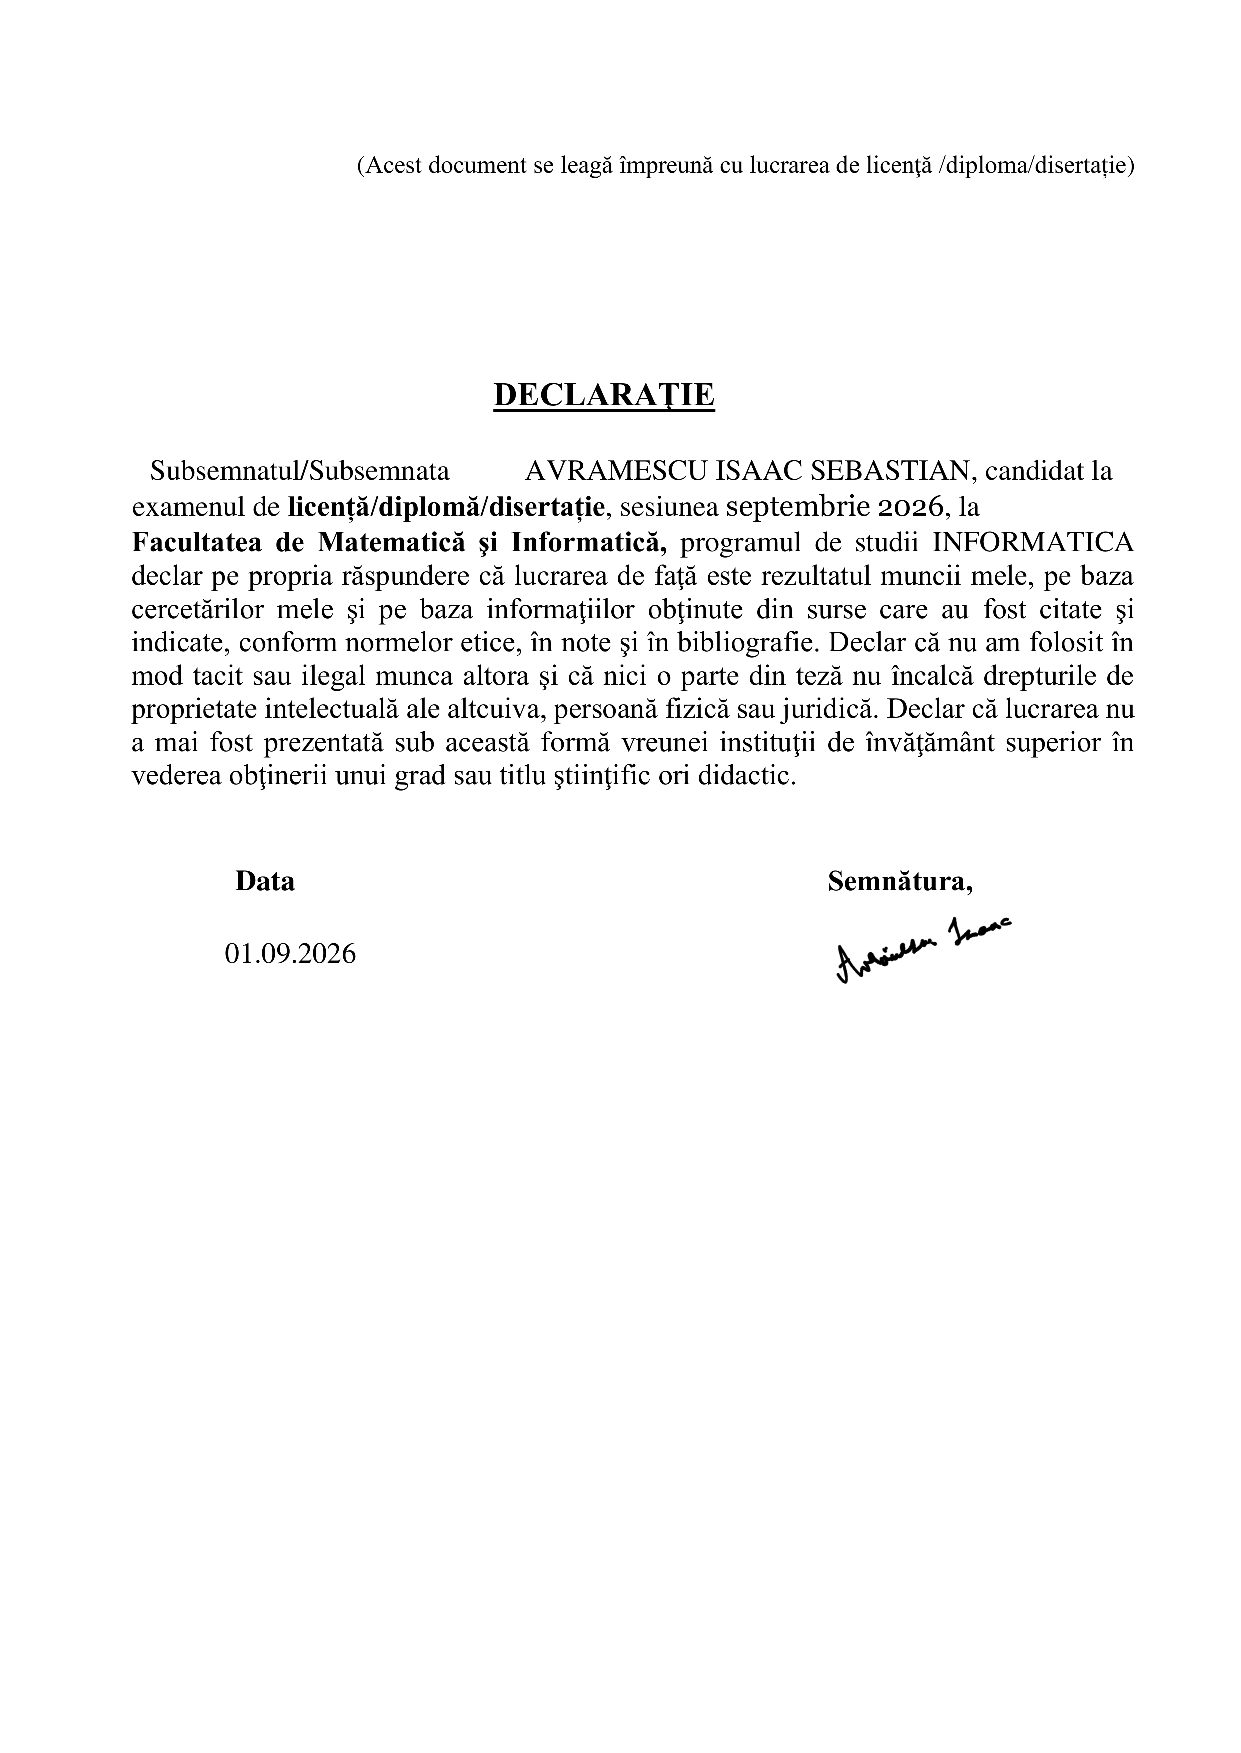
\includepdf[
    pages={1},
    addtotoc={1,chapter,0,Declarație de autenticitate,declaratie},
    pagecommand={\thispagestyle{main}}
]{declaratie-semnata.pdf}


% ----------------------------------------------------------------------------
%  ALTERNATIVĂ (comentată) — dacă vrei în schimb o IMAGINE.
%  Pune fișierul în `images/` și scrie-i numele, fără cale.
% ----------------------------------------------------------------------------

% \addcontentsline{toc}{chapter}{Anexă}
% \chapter*{Anexă}
% \begin{figure}[!ht]
%     \centering
%     \includegraphics[width=\textwidth]{numele-fisierului.png}
%     \caption{Descrierea documentului anexat}
% \end{figure}


\end{document}
